\chapter*{Введение}							% Заголовок
\addcontentsline{toc}{chapter}{Введение}	% Добавляем его в оглавление

\textbf{Актуальность работы}. Системы контроля и управления доступом (СКУД) используются повсеместно, и их количество увеличивается с каждым днем. Обычный дверной замок и соответствующие ему ключи являются примером простейшей СКУД. Более сложными примерами являются системы, основанные на смарт-картах и дверных замках с микроконтроллерами, данные системы широко используются в офисных зданиях и гостиничных комплексах. Еще более сложным примером являются СКУД, основанные на проверке биометрических данных, например, на основе сканирования отпечатка пальцев.

Экспоненциальный рост рынка мобильных устройств с 2007 по 2013 годы открыл перспективы создания СКУД принципиально нового типа, основанных на идеи использовании смартфона в качестве ключа. По данным на начало 2013 года количество смартфонов составляет 22\% от общего населения планеты, при этом среди работающего населения развитых стран этот процент близок к 100\%. Данная статистика свидетельствует о практической возможности внедрения новых мобильных СКУД как для личного, так и для корпоративного сегментов. 

\begin{figure} [h] 
  \center
  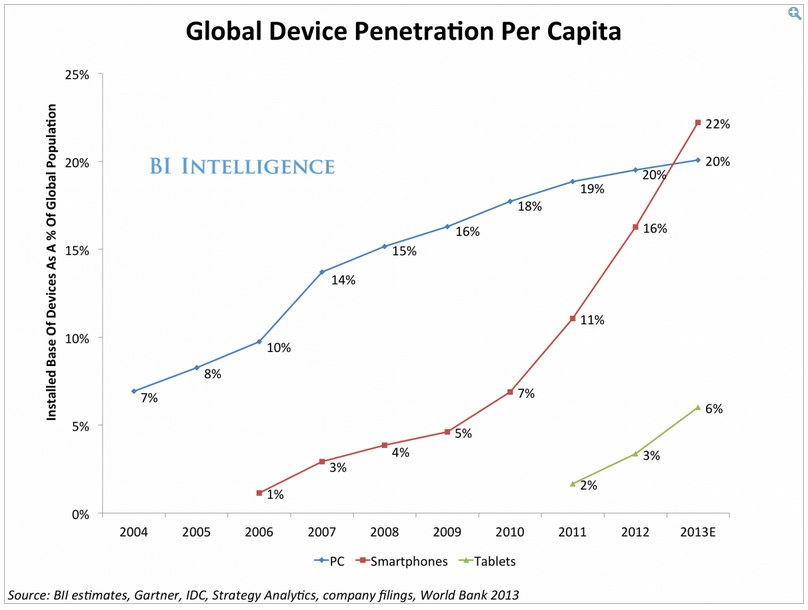
\includegraphics [scale=0.33] {mobile_grow_stat}
  \caption{Рост количества мобильных устройств} 
\end{figure}

Современные мобильные устройства предоставляют разработчикам широкий спектр программно-аппаратных возможностей, и в том числе возможности для захвата базовых биометрических данных пользователя — голоса, внешности и отпечатка пальца. Это позволяет успешно производить биометрическую верификацию пользователя и открывает возможности для создания мобильной биометрической СКУД, реализующей в себе основные преимущества биометрических систем.

Актуальность исследования обуславливается практической значимо­стью и большой востребованностью простых во внедрении, удобных в использовании и безопасных систем контроля доступа. 

\medskip

\textbf{Научная новизна} состоит в создании принципиально новой модели СКУД, реализующей идею использования смартфона в качестве ключа с возможностью биометрической верификации пользователя.

\medskip

\textbf{Объектом исследования} являются системы контроля и управления доступом и возможные пути к увеличению их эффективности, удобства практического использования, надежности и безопасности за счет использования возможностей мобильных устройств и современных технологий.

\medskip

\textbf{Методы исследования}. Для достижения поставленных в диссертационной
работе целей были использованы: теоретический метод, метод моделирования, метод анализа, метод сравнения и метод эксперимента. 

\medskip

\textbf{Цели и задачи диссертации:}
\begin{enumerate}
  \item Разработка новой модели системы контроля и управления доступом в соответствии со сформулированными требованиями.
 
  \item Разработка и подробное описание архитектуры системы и алгоритмов взаимодействия между элементами системы, обеспечивающих целостную безопасность и практическую значимость системы.

  \item Реализация и апробация программного-аппаратного комплекса, реализующего разработанную модель системы контроля доступа и разработанные алгоритмы.
\end{enumerate}

\medskip

\textbf{Достоверность научных положений} подтверждается практической реализацией разработанной модели и ее апробацией в условиях реального предприятия, а также представлением результатов работы на различных научно-практических конференциях.

% хардкордное выравнивание, чтобы текст Основные положения, выносимые на защиту были на той же странице что и список положений
\bigskip
\bigskip
\bigskip

\textbf{Основные положения, выносимые на защиту:}
\begin{enumerate}
  \item Разработанная модель мобильной биометрической системы доступа.
  \item Разработанное прикладное программное-обеспечение, реализующее предложенную модель и алгоритмы взаимодействия.
\end{enumerate}

\medskip

\textbf{Практическая ценность результатов}. Полученная в рамках исследования модель системы доступа представляет большую практическую ценность — так как на ее основе можно успешно создавать промышленные СКУД нового поколения, обеспечивающие высокий уровень безопасности и удобства для конечных пользователей за счет использования возможностей мобильных устройств и современных технологий.

\medskip

\textbf{Область применения результатов.} СКУД, основанные на полученной модели могут быть использованы в различных областях. Краткий список наиболее перспективных и значимых областей применения:
\begin{enumerate}
  \item Жилые дома и квартиры.
  \item Малый и средний бизнес.
  \item Университеты и школы.
  \item Банковские ячейки и камеры хранения.
  \item Гостиничные комплексы.
  \item Домофонные системы.
  \item Коворкинги.
  \item Сервисы аренды автомобилей и проката велосипедов.
\end{enumerate}

\medskip

\textbf{Список публикаций}. На данный момент, материалы диссертации опубликованы в 2 печатных работах, из них 0 статей в журналах из списка, рекомендованного ВАК. 

В 2014 году планируется публикация минимум в 5 российских и европейских научных собраниях, в том числе в 3 журналах из списка, рекомендованного ВАК. 

\medskip

\textbf{Апробация и внедрение результатов}. Результаты работы докладывались на конференциях: <<Всероссийская НПК кафедры АСОИУ>>, г. Омск, ОмГТУ, 2013 год, и <<Интеллектуальные чтения>>, г. Омск, СибАДИ, 2013 год.

В 2014 году планируется выступление на минимум 2 всероссийских научных практических конференциях. Также планируется практическое внедрение системы в нескольких офисах омских компаний и совместно с лабораторией Касперского в рамках проекта умных банковских ячеек.

\medskip

\textbf{Личный вклад автора}. Содержание диссертации и основные поло­жения, выносимые на защиту, отражают персональный вклад автора в опубликованные работы. Все представленные в диссертации результаты по­лучены лично автором.

\medskip

\textbf{Структура и объем диссертации}.

\clearpage